%%%%%%%%%%%%%%%%%%%%%%%%%%%%%%%%%%%%%%%%%
% baposter Portrait Poster
% LaTeX Template
% Version 1.0 (15/5/13)
%
% Created by:
% Brian Amberg (baposter@brian-amberg.de)
%
% This template has been downloaded from:
% http://www.LaTeXTemplates.com
%
% License:
% CC BY-NC-SA 3.0 (http://creativecommons.org/licenses/by-nc-sa/3.0/)
%
%%%%%%%%%%%%%%%%%%%%%%%%%%%%%%%%%%%%%%%%%

%----------------------------------------------------------------------------------------
%	PACKAGES AND OTHER DOCUMENT CONFIGURATIONS
%----------------------------------------------------------------------------------------

\documentclass[a1paper,portrait, fontscale=0.575]{baposter}

\usepackage[font=small,labelfont=bf]{caption} % Required for specifying captions to tables and figures
\usepackage{booktabs} % Horizontal rules in tables
\usepackage{relsize} % Used for making text smaller in some places
% Supports of Russian fonts
\usepackage[T1]{fontenc}
\usepackage[english,russian]{babel}
\usepackage[utf8]{inputenc}
\usepackage{type1ec}
% Math
\usepackage{amsmath,amsthm, amssymb, latexsym}
\usepackage{multicol}

\graphicspath{{figures/}} % Directory in which figures are stored

\definecolor{bordercol}{RGB}{40,40,40} % Border color of content boxes
\definecolor{headercol1}{RGB}{186,215,230} % Background color for the header in the content boxes (left side)
\definecolor{headercol2}{RGB}{80,80,80} % Background color for the header in the content boxes (right side)
\definecolor{headerfontcol}{RGB}{0,0,0} % Text color for the header text in the content boxes
%\definecolor{boxcolor}{RGB}{186,215,230} % Background color for the content in the content boxes
\definecolor{boxcolor}{RGB}{255,255,255}
\begin{document}
    
    \background{ % Set the background to an image (background.pdf)
        %\begin{tikzpicture}[remember picture,overlay]
        %\draw (current page.north west)+(-2em,2em) node[anchor=north west]
        %{
\includegraphics[height=1.1\textheight]{background}};
        %\end{tikzpicture}
    }
    
    \begin{poster}{
            %grid=true,
            borderColor=bordercol, % Border color of content boxes
            headerColorOne=headercol1, % Background color for the header in the content boxes (left side)
            headerColorTwo=headercol2, % Background color for the header in the content boxes (right side)
            headerFontColor=headerfontcol, % Text color for the header text in the content boxes
            boxColorOne=boxcolor, % Background color for the content in the content boxes
            headershape=roundedright, % Specify the rounded corner in the content box headers
            headerfont=\Large\sf\bf, % Font modifiers for the text in the content box headers
            textborder=rectangle,
            background=user,
            headerborder=open, % Change to closed for a line under the content box headers
            boxshade=plain
        }
        {}
        %
        %----------------------------------------------------------------------------------------
        %	TITLE AND AUTHOR NAME
        %----------------------------------------------------------------------------------------
        %
        {\sf\bf Проектирование детектора солнечных космических лучей} % Poster title
        {\vspace{1em} Е. Стадничук$^{1,2}$, М. Зелёный$^{1,2,3}$, А. Нозик$^{1,2}$, И. Зимовец$^{3}$
            \\ % Author names
            {\smaller egrstadnichuk@yandex.ru, mihail.zelenyy@phystech.edu }
            \\
            {\smaller $^1$МФТИ (НИУ), $^2$ИЯИ РАН, $^3$ИКИ РАН }
            \\
            {\smaller Четырнадцатая ежегодная конференция <<Физика плазмы в солнечной системе>>, 11-15 февраля, 2019}
        } % Author email addresses
        {
\includegraphics[scale=1]{logoNpm.pdf}} % University/lab logo
        
        
        %----------------------------------------------------------------------------------------
        %	INTRODUCTION
        %----------------------------------------------------------------------------------------
        
        \headerbox{Введение}{name=introduction,column=0,row=0}{
            
            Актуальными задачами в космосе являются:
            \begin{itemize}
                \item Проведение исследований солнечных космических лучей и солнечных вспышек;
                \item Обеспечение радиационной безопасности для космонавтов и электроники.
            \end{itemize}
            \\
            Для решения этих задач необходимы детекторы:
            \begin{itemize}
                \item Регистрирующие протоны с энергией от 10 МэВ до 100 МэВ
                и электроны с энергией от 1 МэВ до 10 МэВ;
                \item Работающие в условиях больших ($>10^6$ Гц) загрузок и узких каналов связи;
                \item Имеющие оптимальные масса-габаритные характеристики
            \end{itemize}
        }
        
        \headerbox{Конструкция детектора}{name=prototype,span=1,column=0,below=introduction, above=bottom}{
            \begin{center}
                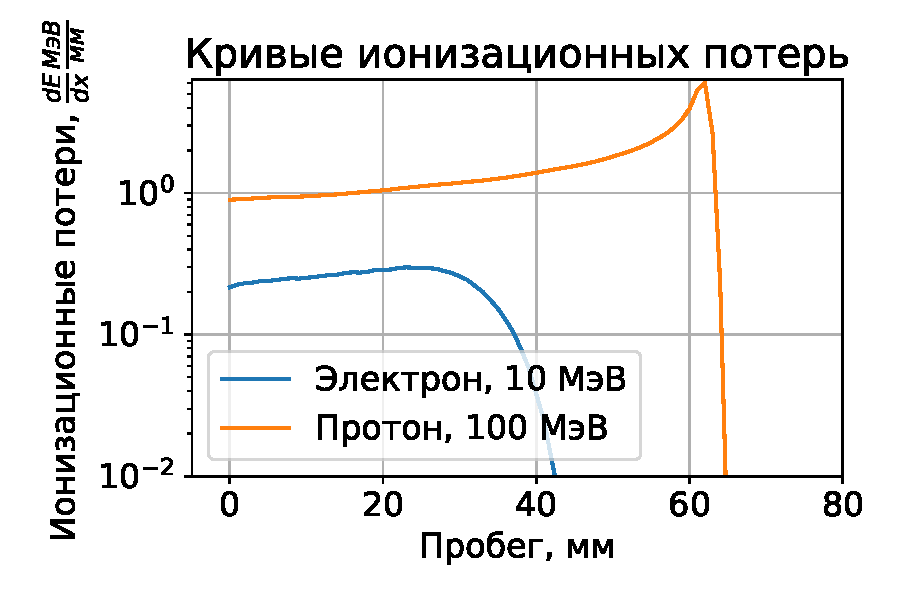
\includegraphics[width=0.8\linewidth]{01_bregg.pdf}
                \captionof{figure}{Кривые ионизационных потерь для протона и электрона.}
                \label{bragg}
            \end{center}
            Принцип регистрации частиц основан на измерении потерь в веществе детктора. Тип частицы, начальную кинетическую энергию и угол влета можно восстановить по кривой потерь (рис.~\ref{bragg}).
            
            Детектор представляет собой цилиндр, собранный из нескольких сцинтилляционных дисков (рис.~\ref{device}). Диски распологаются по возрастанию толщины: от более тонких (обеспечивающих регистрацию электронов) на входе до более толстых на конце детектора (работающих при прохождении высокоэнергитичных протонов). 
            
            \begin{center}
                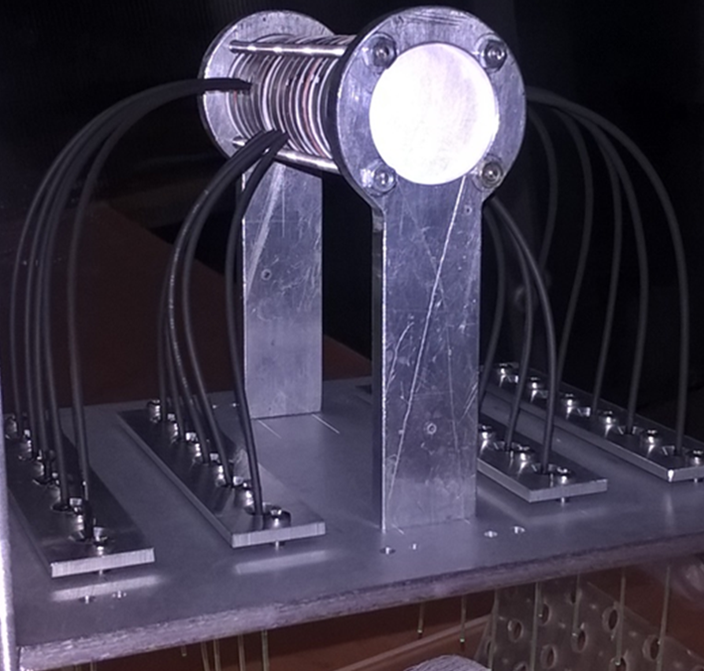
\includegraphics[width=0.9\linewidth]{detector.png}
                \captionof{figure}{Макет протонной части детектора.}
                \label{device}
            \end{center}   
            Данная геометрия дает следующие преимущества:
            \begin{itemize}
                \item Проводится измерение пространственного распределения энерговыделения в детекторе, что позволяет получить больше информации о частице;
                \item Обеспечивается вариативность прибора: характеристики прибора легко регулируются заменой одного или нескольких сцинтилляционных дисков;
                \item Обеспечивается модульность прибора: сцинтилляционные диски могут быть объедены в кассеты, решающие конкретные задачи.
            \end{itemize}  
            %    Прототип детектора имеет следующую конструкцию . Шайбы сцинтиллятора соединяются в цилиндр и удерживаются с помощью четырех стержней и двух металических пластин, имеющих входное окно. С помощью ножек цмлмндр крепится на основную плату. К плате снизу присоединена электроника, на которой располагаются SiPM (рисунок~\ref{electronic}). Из сцинтилляторов выведено оптоволокно, которое крепится непосредственно к MPPC.
            
            \begin{center}
                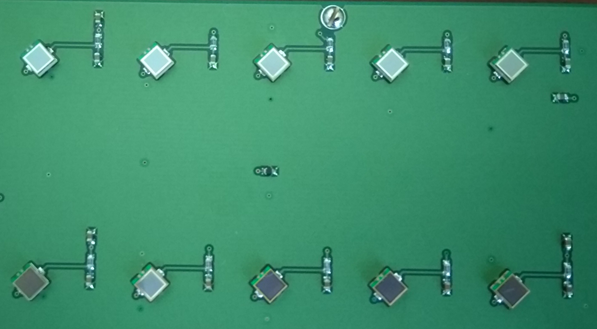
\includegraphics[width=0.85\linewidth]{electronics.png}
                \captionof{figure}{Электроника для считывания сигнала с детектора.}
                \label{electronic}
            \end{center}
            Для улучшения разрешающих и массовых характеристик детекторов предлагается использовать MPPC вместо классических ФЭУ.
        }
        
        
        
        \headerbox{Восстановление сигнала}{name=method,span=2,column=1}{
            \begin{multicols}{2}
                \begin{center}
                    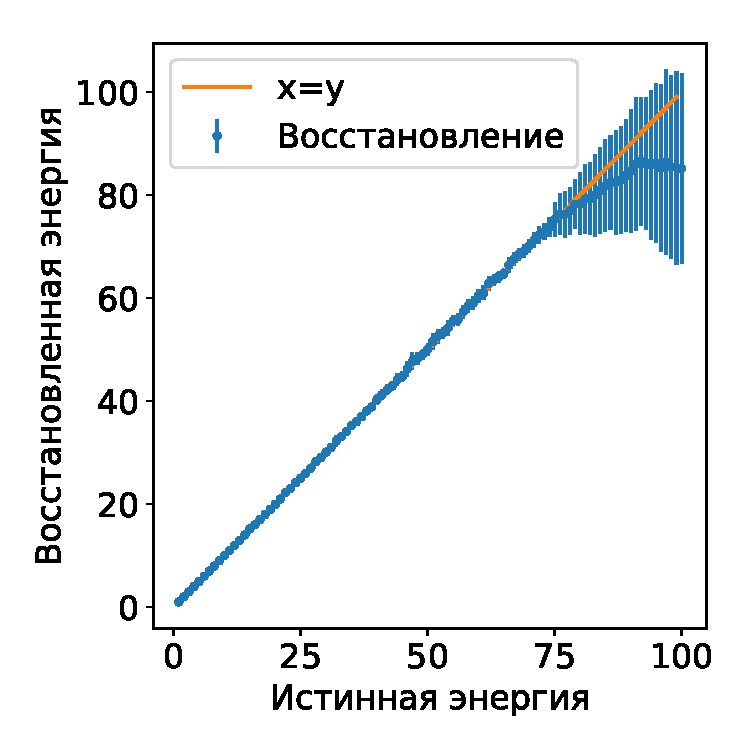
\includegraphics[width=0.6\linewidth]{resolution.pdf}
                    \captionof{figure}{Моделирование восстановления в счетном режиме.}
                    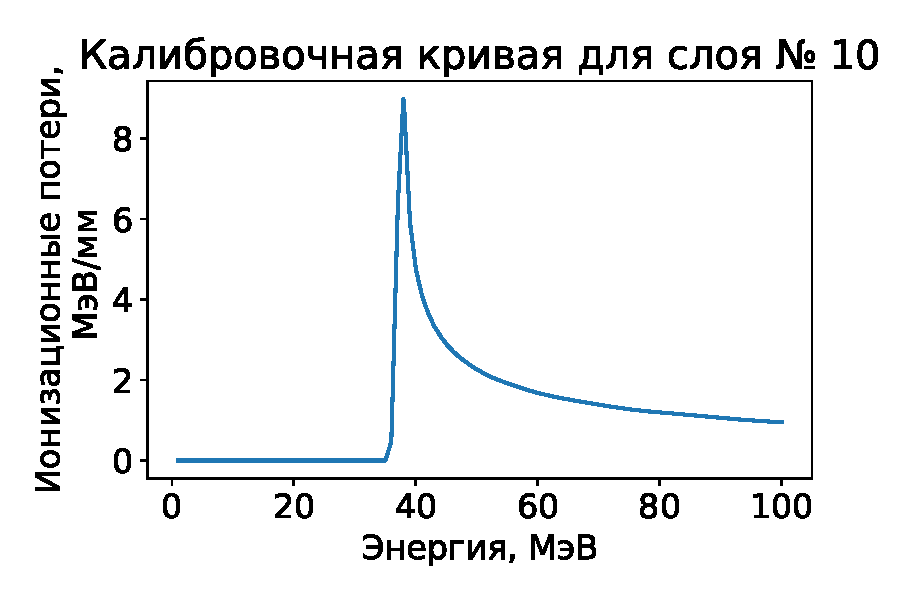
\includegraphics[width=0.9\linewidth]{Calibration.pdf}
                    \captionof{figure}{Пример калибровочной кривой для статистической регуляризации Турчина.}
                \end{center}
            \end{multicols}
            \begin{multicols}{2}
                Высокие характеристики прибора и возможность работь в сложных условиях обеспечиваются не только оригинальной конструкцией, но и использованием продвинутых алгоритмов анализа данных.\\
                \vfill\null
                \columnbreak
                Исследуется возможность работы прибора в двух режимах:
                \begin{itemize}
                    \item Счетном или одночастичный режим, когда анализируется каждая частица попавшая в детектор;
                    \item Интегральный --- когда анализируется суммарное энерговыделение от большого числа частиц и восстанавливается их спектр. Анализ в данном режиме основан на статистической регуляризации Турчина.
                \end{itemize}
                
            \end{multicols}
            
            \begin{center}
                
                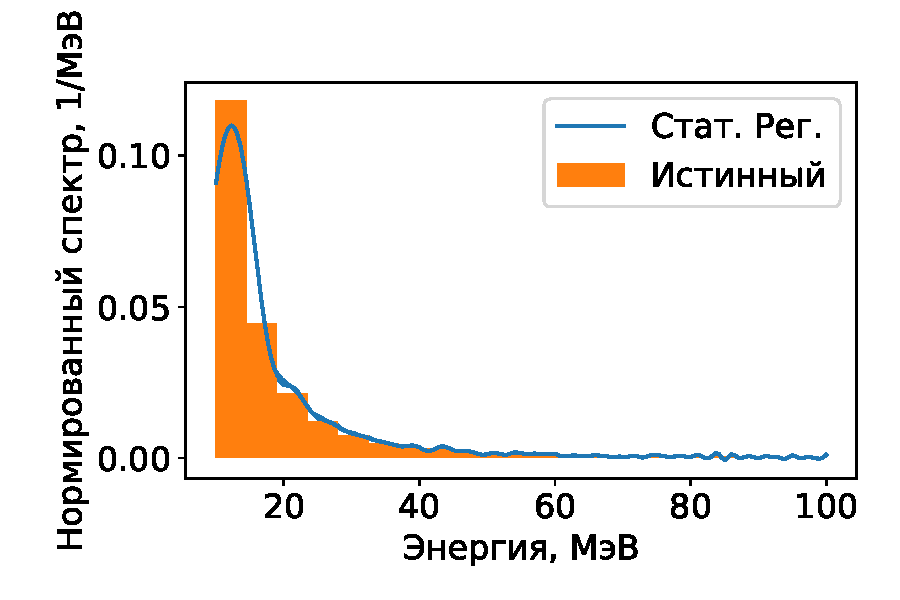
\includegraphics[width=0.45\linewidth]{Pow.pdf}
                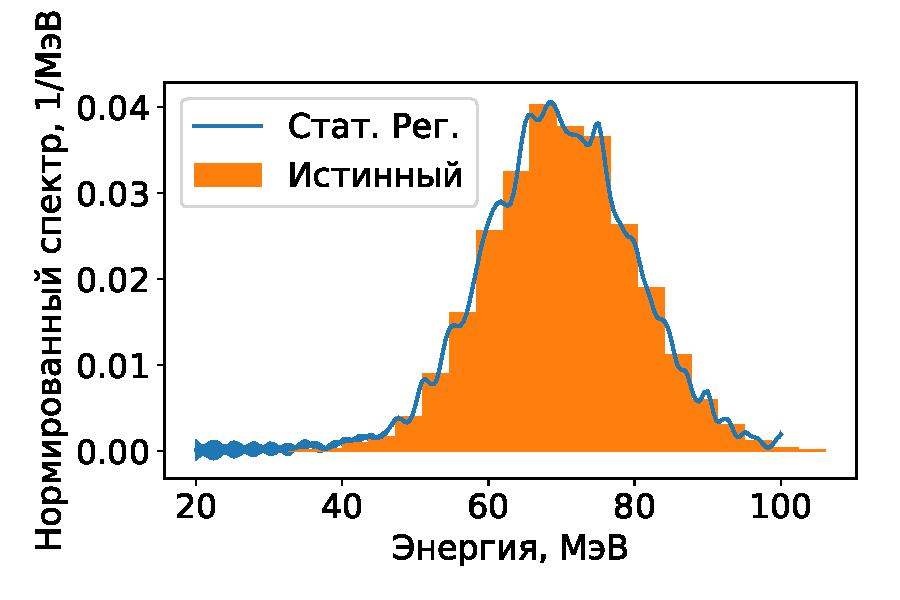
\includegraphics[width=0.45\linewidth]{Gauss.pdf}
                
                \captionof{figure}{Моделирование восстановления спектров с помощью статистической регуляризации Турчина.}  
            \end{center}
        }
        
        %----------------------------------------------------------------------------------------
        %	Анализ светосбора
        %----------------------------------------------------------------------------------------
        \headerbox{Крепление MPPC}{name=lightcollect,span=1,column=1, below= method}{
            
            Свет с сцинтиллятора регистрируется с помощью MPPC (Hamamatsu SiPM S12575-015P). Закрепить на сцинтилляторе их можно двумя способами (рис.~\ref{lightcollect1} и рис.~\ref{lightcollect2}) 
            %------------------------------------------------
            \begin{multicols}{2}
                \begin{center}
                    %        Возможные способы крепления MPPC к шайбе детектора.
                    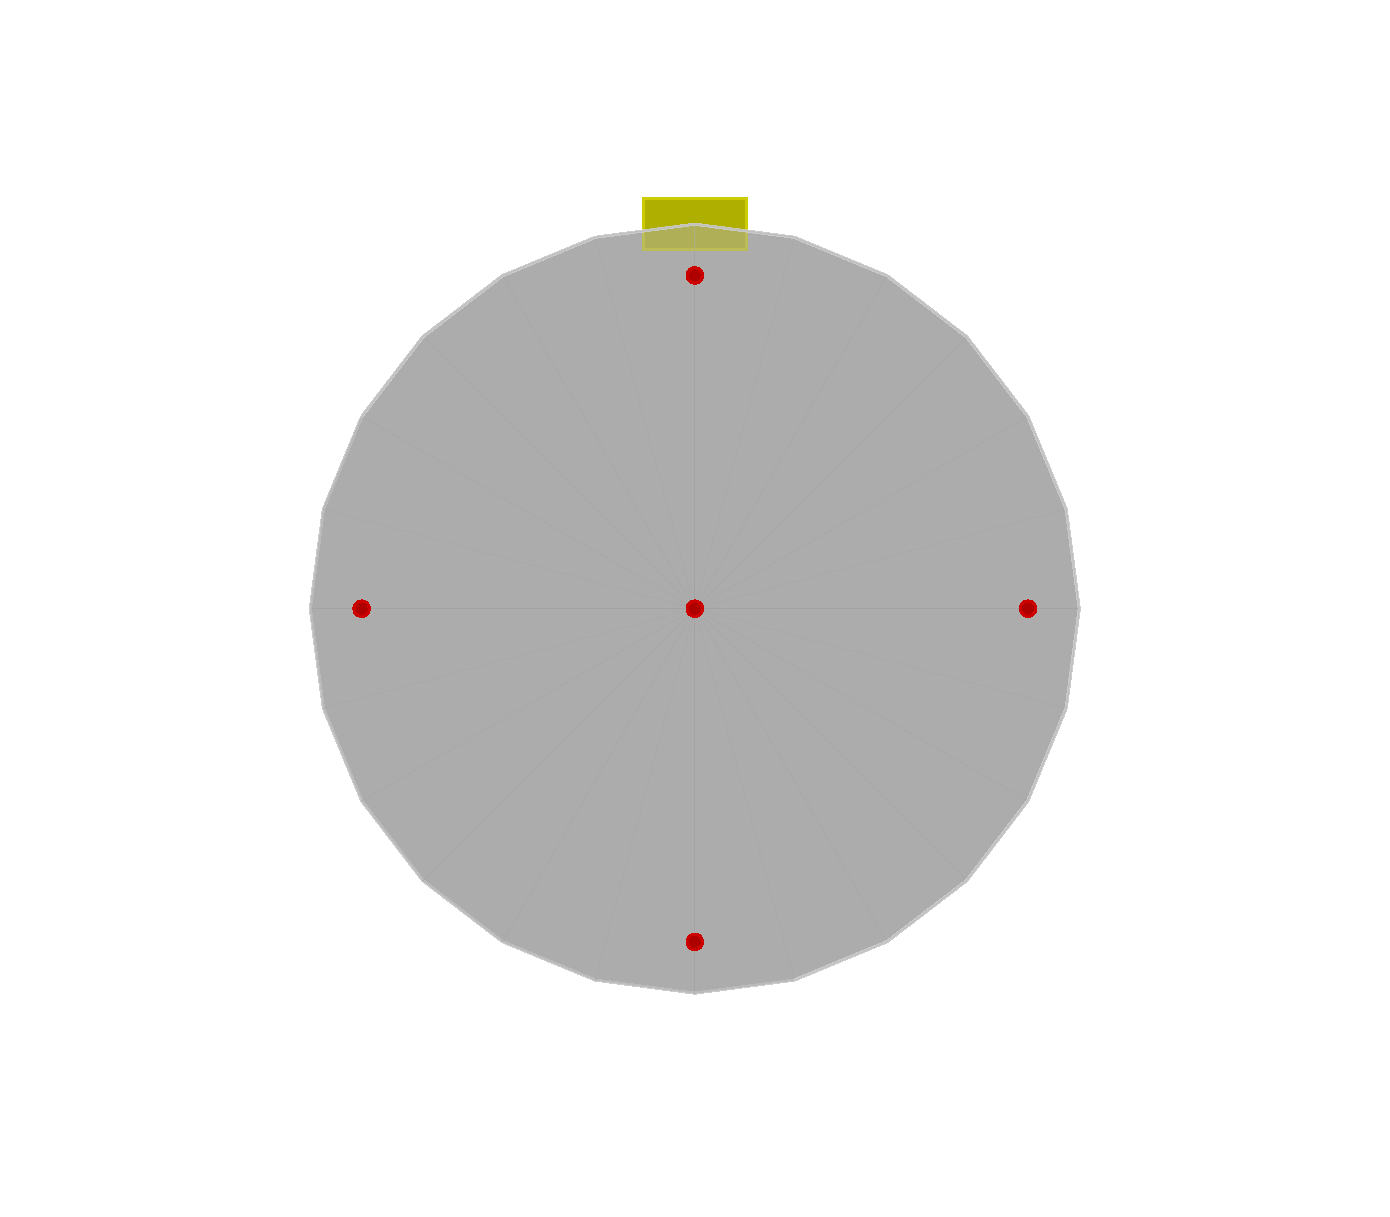
\includegraphics[width=0.9\linewidth]{light_2.pdf}
                    \captionof{figure}{ Прикрепление MPPC непосредственно к сцинтиллятору.}
                    \label{lightcollect1}
                    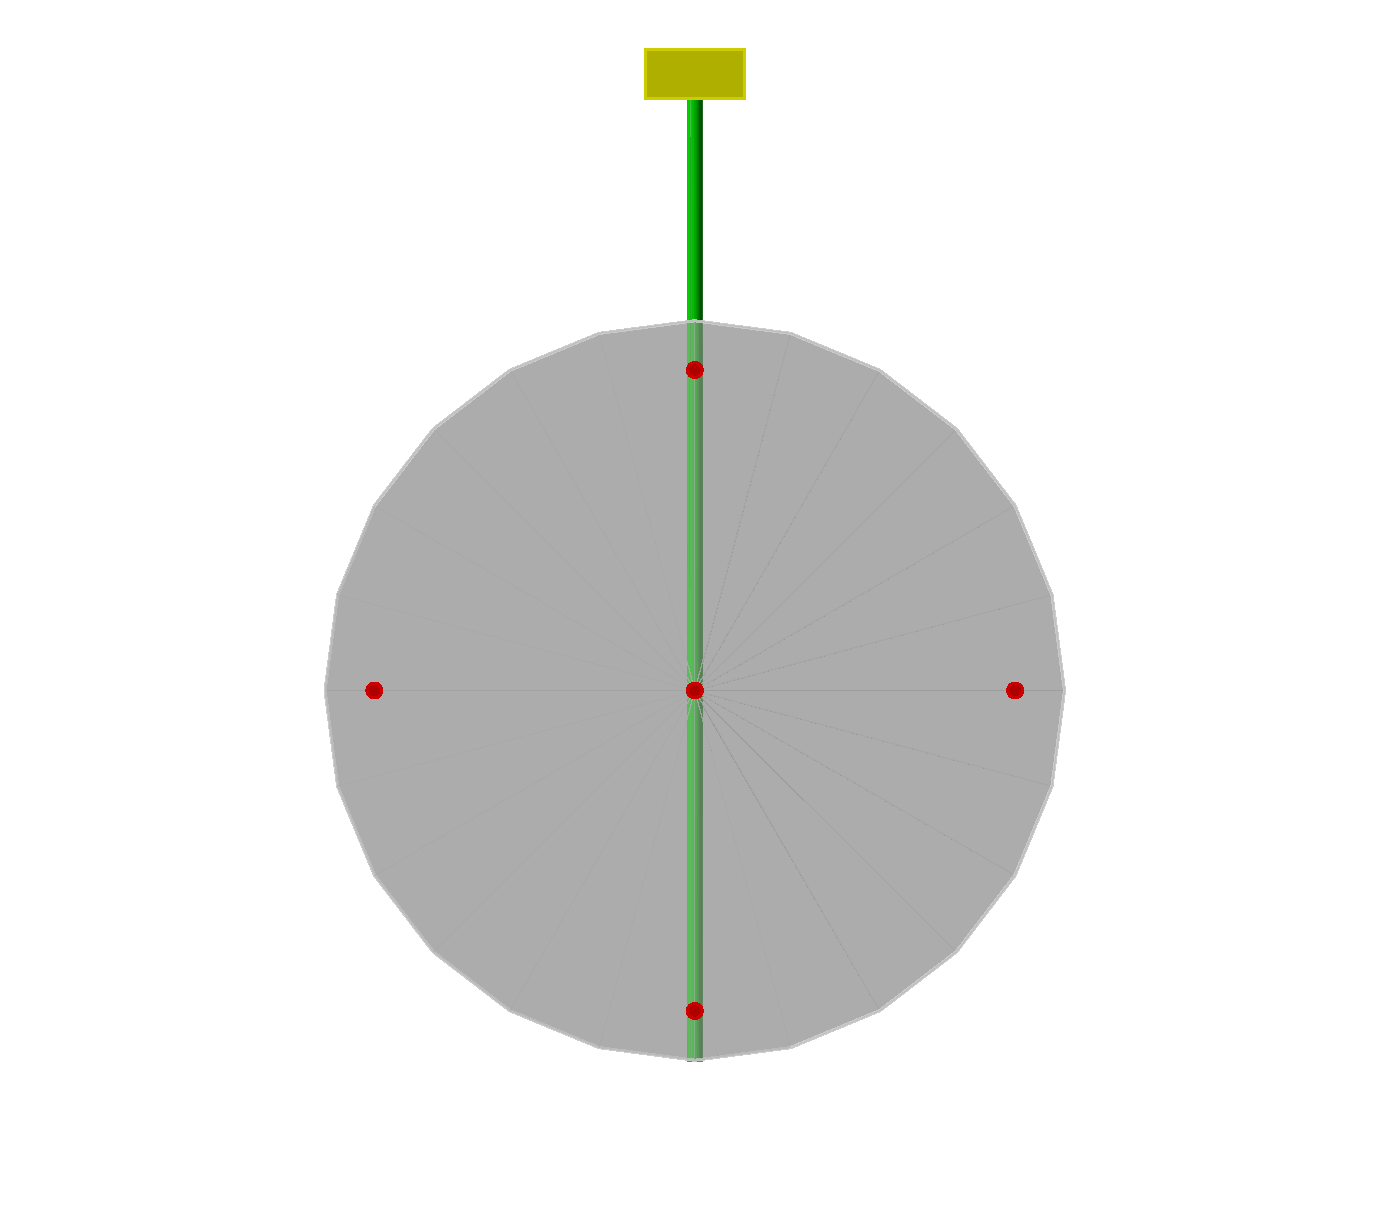
\includegraphics[width=0.9\linewidth]{light_1.pdf}
                    \captionof{figure}{Снятие света внутри сцинтиллятора оптоволокном и вывод его на MPPC.}
                    \label{lightcollect2}
                    
                \end{center}
            \end{multicols}
            %------------------------------------------------
            Для того, чтобы выбрать конкретный способ для каждого случая, в точках, отмеченных красным, был размещен $\beta$-источник и были измерены:  
            \begin{itemize}
                \item{Светосбор (определяет амплитуду сигнала на MPPC на единицу энергии, потерянной частицей в шайбе);}
                \item{Однородность светосбора (определяет, как сигнал зависит от точки входа частицы в шайбу).}
            \end{itemize}
            В результате оказалось, что:
            \begin{itemize}
                \item{Количество фотоэлектронов в первом случае в три раза больше чем во втором; }
                \item{Разница в количестве фотоэлектронов, регистрируемых для частиц, попадающих в центр и в край сцинтиллятора, равна 40\% для первого случая и 7\% --- для второго. }
            \end{itemize}
            Конструкция с оптоволокном обладает практически полной однородностью светосбора и гораздо удобнее в эксплуатации, поэтому  используется при сборке детектора.
            
        }
        
        \headerbox{Влияние температуры}{name=temp,span=1,column=2,below =method}{
            MPPC Hamamatsu SiPM S12575-015P рассчитаны на работу при температурах от $-20~^\circ C$ до $+50~^\circ C$, однако для оптимальной работы требуется подстройка подаваемого напряжения.    В документации SiPM приведена зависимость оптимального напряжения от температуры, но в рамках данной работы эта зависимость была проверена экспериментально (рис.~\ref{temp}).
            \begin{center}
                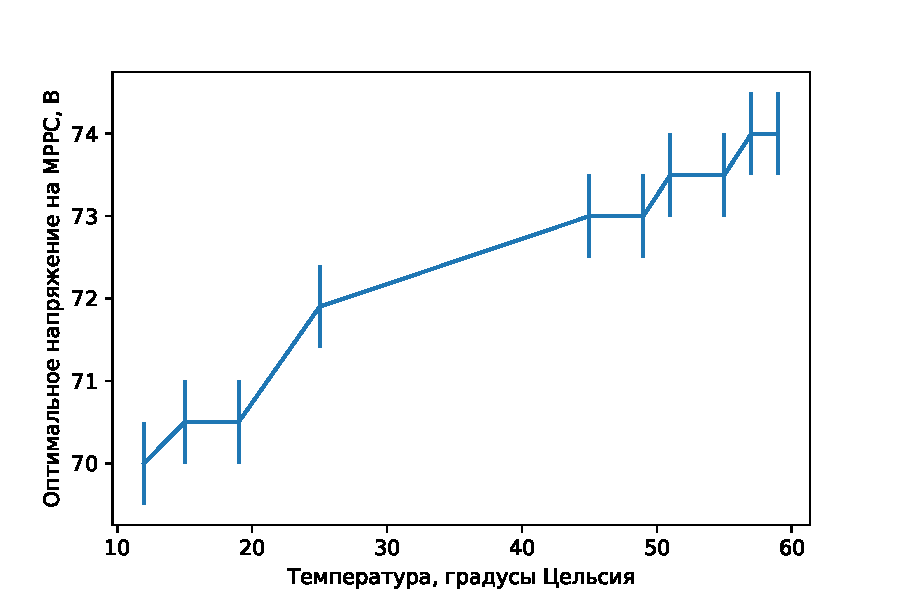
\includegraphics[width=0.9\linewidth]{optimal_voltage.pdf}
                \captionof{figure}{Оптимальное напряжение на MPPC в зависимости от температуры}
                \label{temp}
            \end{center}
            Отсюла следует, что в конструкции детектора должен быть предусмотрен термодатчик для корректировки напряжения на MPPC (для испытаний макета используется термопара и система Slow Control).
        }
        
        \headerbox{Результаты}{name=conclusion,column=1,below=lightcollect, above=bottom}{
            \begin{itemize}
                \item Спроектирован детектор солнечных космических лучей;
                \item Собран макет детектора;
                \item Проверена зависимость работы MPPC от температуры;
                \item Разработана методика анализа данных.
            \end{itemize}
            Работа сделана при поддержке гранта РНФ 17-72-20134.
            %~\cite{petrukovich2008cosmic}  
        }
        
        
        \headerbox{Список литературы}{name=references,column=2,below=temp, above=bottom}{
            
            \smaller % Reduce the font size in this block
            \renewcommand{\section}[2]{\vskip 0.05em} % Get rid of the default "References" section title
            \nocite{*} % Insert publications even if they are not cited in the poster
            
            \bibliographystyle{unsrt}
            \bibliography{references} % Use sample.bib as the bibliography file
        }
        
    \end{poster}
    
\end{document}